\documentclass[aspectratio=169]{beamer}
\usetheme{moloch}           % Use metropolis theme

% tables
\usepackage{adjustbox}
\usepackage{longtable}
\usepackage{booktabs}
\usepackage{ltablex}
\keepXColumns  % evita che LaTeX sostituisca X con p{}

% graphics
\usepackage{graphicx}

% citations and bibliography
% \usepackage{babel}[English] % Use English language
\usepackage{csquotes}
\usepackage{caption}
\usepackage{subcaption}

\usepackage[backend=biber,style=authoryear]{biblatex}
\addbibresource{Tesi-triennale.bib}
 % Load custom preamble with packages and settings

\title{AWB algorithms and dataset comparison}
\date{\today}
\author{Alessandro Teodori}
% \institute{Centre for Modern Beamer Themes}
\begin{document}
  \maketitle
  \section{AWB algorithms}
    \begin{frame}
      % Tabella 3.1a - Caratteristiche Principali
\begin{table}[htbp]
\centering
\caption{Caratteristiche principali degli algoritmi di stima dell'illuminante}
\label{tab:algorithms}
\footnotesize
\begin{tabularx}{\textwidth}{lccccXl}
\toprule
\textbf{Algoritmo} & \textbf{Tipo} & \textbf{Illum.} & \textbf{Categ.} & \textbf{Space} & \textbf{Perf.} & \textbf{Ref.} \\
\midrule
\multicolumn{7}{l}{\textit{Metodi Tradizionali}} \\
\midrule
Gray World & img & glob. & trad. & RGB & media & \cite{zapryanov_automatic_2012} \\
AGWM & img & glob. & trad. & RGB & media & \cite{weng_novel_2005} \\
White Patch & img & glob. & trad. & RGB & buona* & \cite{zapryanov_automatic_2012} \\
Gray Edge & img & glob. & trad. & RGB & buona & \cite{van_de_weijer_edge-based_2007} \\
Shades of Gray & img & glob. & trad. & RGB & buona & \cite{zapryanov_automatic_2012} \\
Greyness WA & img & glob. & trad. & YCbCr & alta & \cite{thai_fast_2016} \\
GCP-AWB & img & local & trad. & YUV & buona & \cite{huo_robust_2006} \\
\midrule
\multicolumn{7}{l}{\textit{Metodi Avanzati e Machine Learning}} \\
\midrule
FFCC & img & glob. & ibr. & log-chr. & altiss. & \cite{barron_fast_2017} \\
IFFCC & video & spat.v. & ibr. & log-chr. & altiss. & \cite{wei_integral_2025} \\
KNN-WB & img & glob. & ML & sRGB & media & \cite{afifi_deep_2020} \\
Deep WB & img & glob. & DL & sRGB & alta & \cite{afifi_deep_2020} \\
Deep WB Blend. & img+vid & spat.v. & DL & sRGB & alta & \cite{afifi_auto_2022} \\
\bottomrule
\end{tabularx}
\end{table}

% Tabella 3.1b - Dettagli Implementativi
\begin{table}[htbp]
\centering
\caption{Dettagli implementativi degli algoritmi (continua dalla Tabella \ref{tab:algorithms})}
\footnotesize
\begin{tabularx}{\textwidth}{l>{\raggedright\arraybackslash}Xl>{\raggedright\arraybackslash}X>{\raggedright\arraybackslash}X}
\toprule
\textbf{Algoritmo} & \textbf{Assunzioni Principali} & \textbf{Compl.} & \textbf{Input Richiesti} & \textbf{Estensioni} \\
\midrule
\multicolumn{5}{l}{\textit{Metodi Tradizionali}} \\
\midrule
Gray World & Colore medio grigio & bassa & nessuno & Gray Edge et al. \\
AGWM & Esclude pixel saturi & bassa & nessuno & versioni local \\
White Patch & Pixel più luminoso bianco & bassa & nessuno & filtri anti-rumore \\
Gray Edge & Media gradienti grigia & media & derivate & ordini/pesi \\
Shades of Gray & Estens. GW con $L^p$ & media & parametro $p$ & tuning $p$ \\
Greyness WA & Pixel grigi pesati Cb+Cr & medio-bassa & nessuno & downsampling \\
GCP-AWB & Punti grigi dev. min. U,V & bassa & nessuno & soglia adatt. \\
\midrule
\multicolumn{5}{l}{\textit{Metodi Avanzati e Machine Learning}} \\
\midrule
FFCC & Stima torus log-chroma FFT & molto bassa & nessuno & smooth. temp. \\
IFFCC & Log-chroma illum. locale & molto bassa & nessuno & guided filt. \\
KNN-WB & Inferisce WB da simili KNN & media & dataset sRGB & accelerabile \\
Deep WB & Encoder-decoder DNN AWB & medio-alta & nessuno & edit in/out \\
Deep WB Blend. & Fonde img diversi WB DNN & alta & preset WB & preset var. \\
\bottomrule
\end{tabularx}
\end{table}

    \end{frame}
  \section{Datasets}
    \begin{frame}
      % Tabella 3.2a - Informazioni Generali
\begin{table}[htbp]
\centering
\caption{Informazioni generali sui dataset per la stima dell'illuminante}
\label{tab:datasets}
\footnotesize
\begin{tabularx}{\textwidth}{lccXccl}
\toprule
\textbf{Nome} & \textbf{Scena} & \textbf{Illum.} & \textbf{Ground Truth} & \textbf{N. Img} & \textbf{Disp.} & \textbf{Ref.} \\
\midrule
\multicolumn{7}{l}{\textit{Dataset Single-Illuminant}} \\
\midrule
Color Checker & in+out & single & Macbeth ColorChecker & 568 & pubb. & \cite{gehler_bayesian_2008} \\
Cube++ & in+out & single & Macbeth ColorChecker & 1365 & pubb. & \cite{ershov_cube_2020} \\
INTEL-TAU & in+out & single & RAW + ColorChecker & 7022 & pubb. & \cite{laakom_intel-tau_2020} \\
NUS 8-Camera & in+out & single & Macbeth ColorChecker & 1736 & pubb. & \cite{cheng_illuminant_2014} \\
\midrule
\multicolumn{7}{l}{\textit{Dataset Multi-Illuminant}} \\
\midrule
Beigpour Multi-I. & indoor & multi & per-pixel completo & ~1500 & pubb. & \cite{beigpour_multi-illuminant_2013} \\
SFU Gray Sphere & in+out & multi & gray sphere in frame & 11000 & pubb. & \cite{aghaei_flying_2020} \\
LSMI & indoor & multi & per-pixel mixing & 7486 & pubb. & \cite{kim_large_2021} \\
Flying Gray Ball & indoor & multi & per-pixel sparso & 1300 & pubb. & \cite{ciurea_large_2003} \\
\bottomrule
\end{tabularx}
\end{table}

% Tabella 3.2b - Specifiche Tecniche
\begin{table}[htbp]
\centering
\caption{Specifiche tecniche dei dataset (continua dalla Tabella \ref{tab:datasets})}
\footnotesize
\begin{tabularx}{\textwidth}{ll>{\raggedright\arraybackslash}Xl>{\raggedright\arraybackslash}X}
\toprule
\textbf{Nome} & \textbf{Formato} & \textbf{Camere} & \textbf{Risoluzione} & \textbf{Annotazioni Extra} \\
\midrule
\multicolumn{5}{l}{\textit{Dataset Single-Illuminant}} \\
\midrule
Color Checker & RAW+TIFF & Canon 1D, 5D & 3504$\times$2336 / 4368$\times$2912 & RGB, WB mult., chart \\
Cube++ & RAW+sRGB & Canon EOS 550D & 5184$\times$3456 & bbox, RGB, preview \\
INTEL-TAU & TIFF 16bit & Canon 5DSR, Nikon D810, Sony IMX135 & var. alta ris. & RGB, GDPR, spettro \\
NUS 8-Camera & RAW & 8 camere diverse & variabile & cross-camera GT \\
\midrule
\multicolumn{5}{l}{\textit{Dataset Multi-Illuminant}} \\
\midrule
Beigpour Multi-I. & RAW+sRGB & Nikon D300 + Kinect & 4288$\times$2848 + VGA & refl., shading, depth \\
SFU Gray Sphere & JPEG/PNG & Sony VX-2000 & ~720$\times$480 & dominant+second. RGB \\
LSMI & RAW & Note20 Ultra, $\alpha$9, D810 & variabile & mixing maps, CC \\
Flying Gray Ball & RAW+TIFF & Canon 5D Mk II & 5616$\times$3744 & coord ball, segment. \\
\bottomrule
\end{tabularx}
\end{table}

    \end{frame}
    
    \begin{frame}
    \frametitle{beigpour multi-illuminant}
      
      \begin{figure}[h]
        \centering
        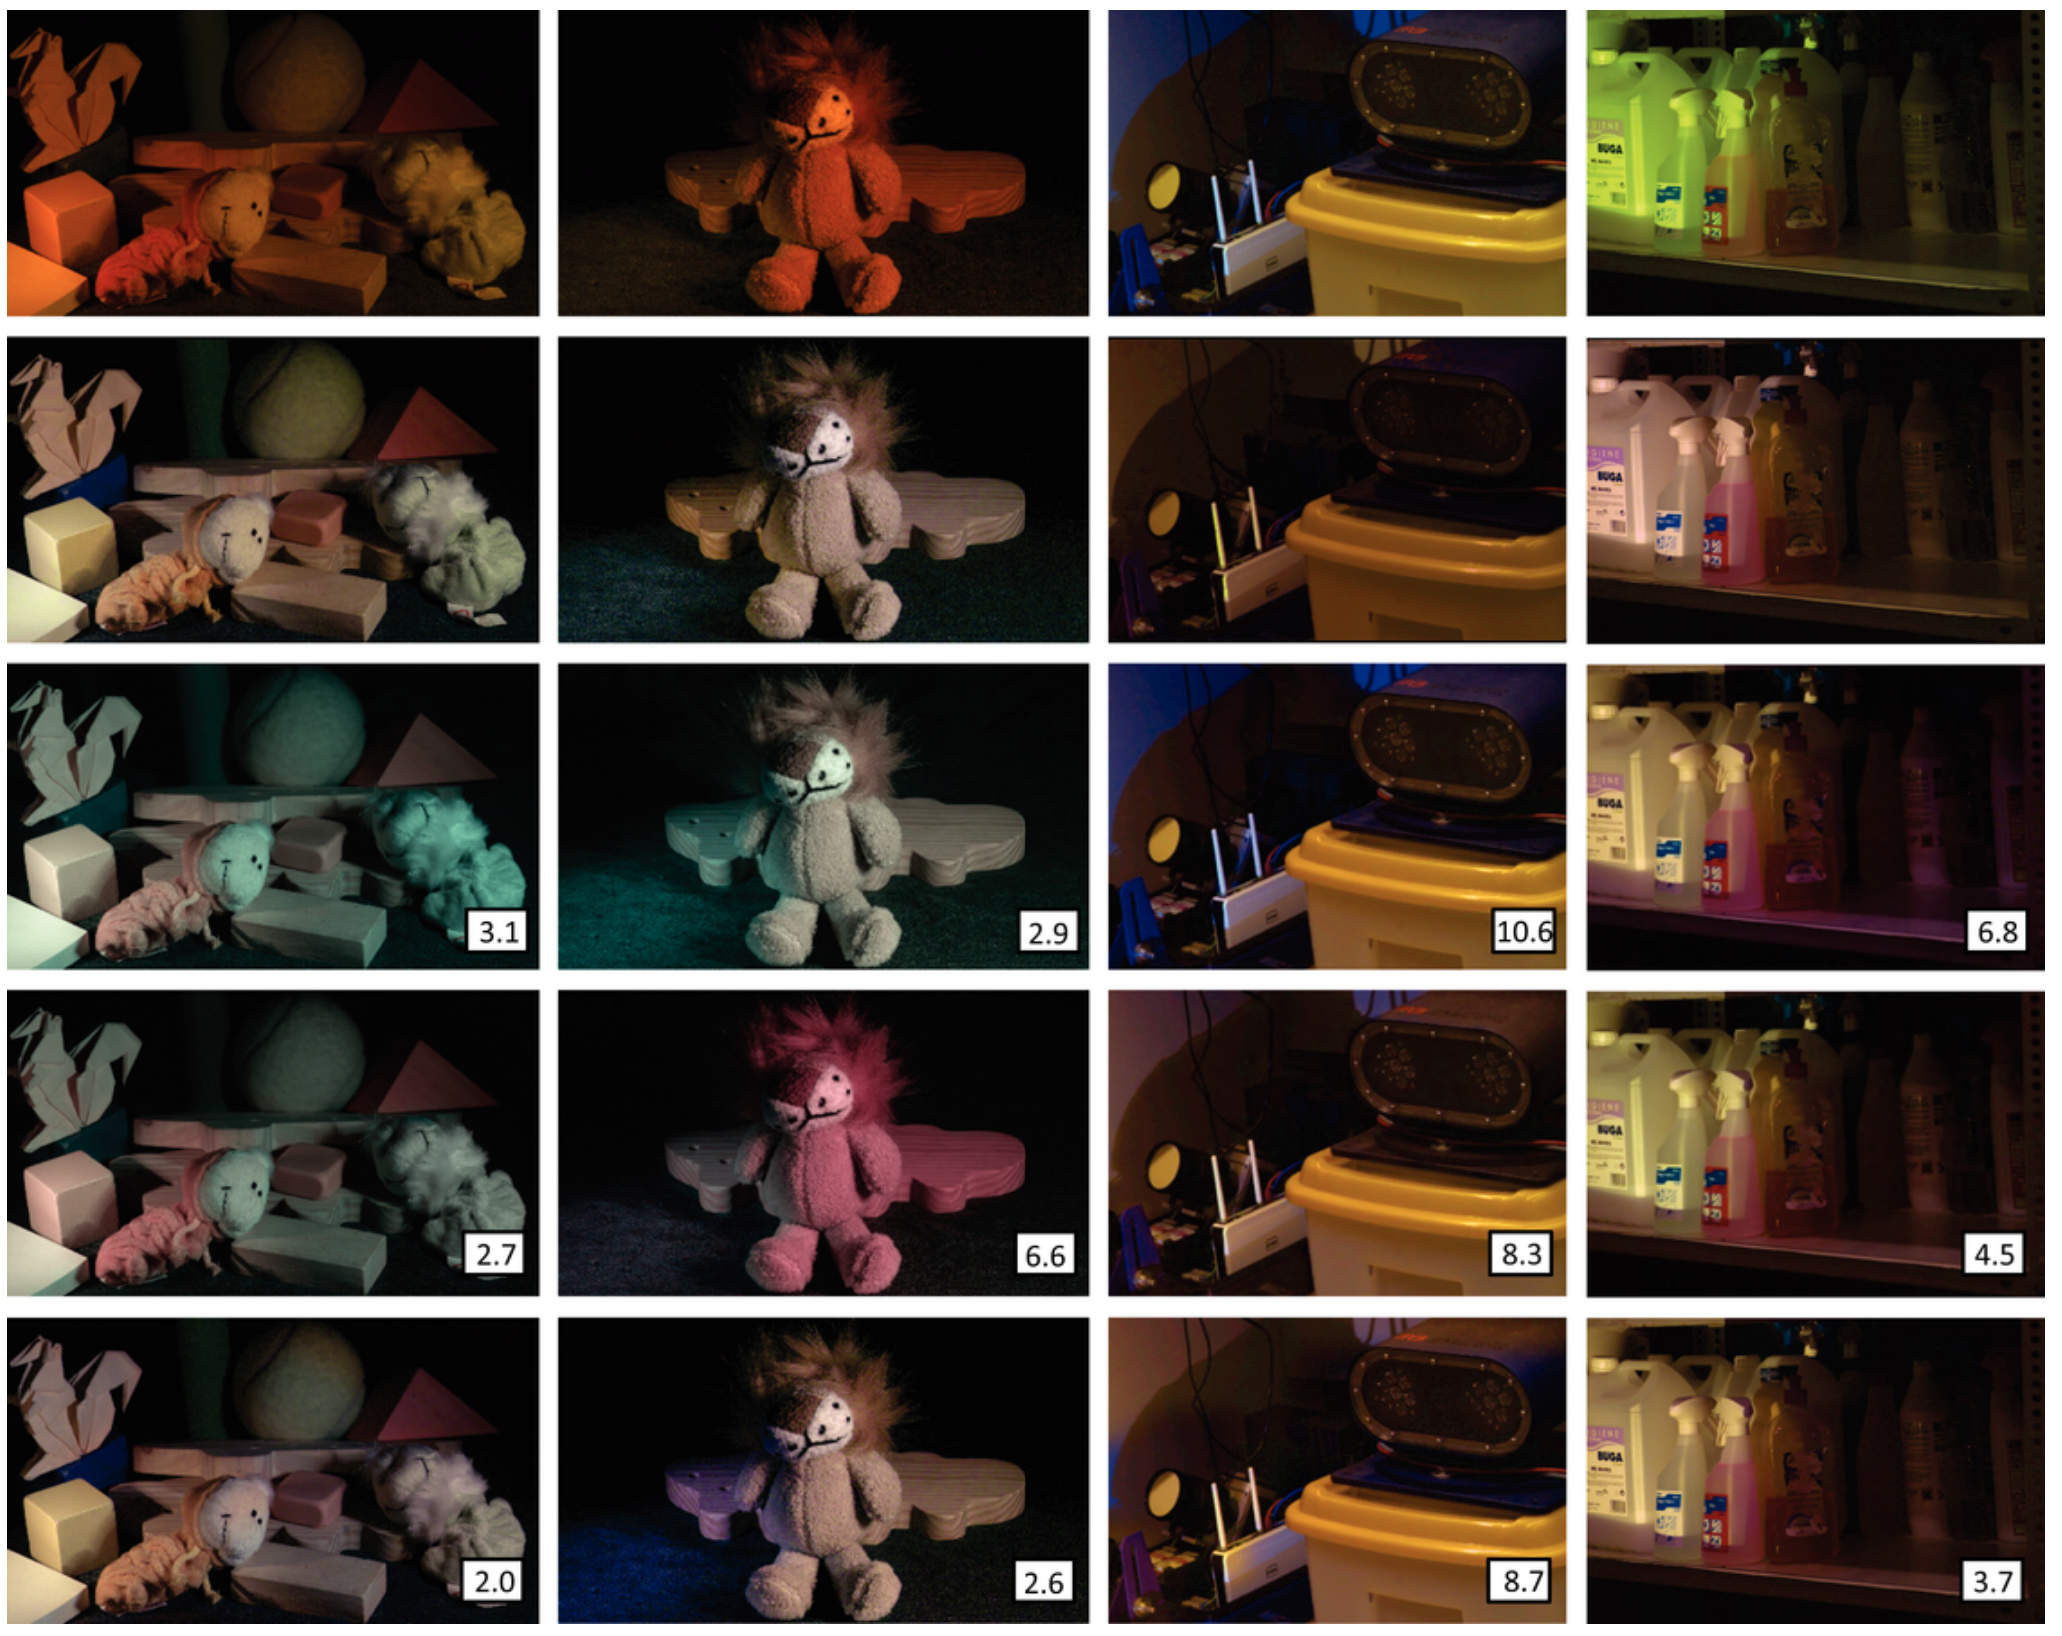
\includegraphics[width=0.5\textwidth]{img/beigpour-dataset-sample.png}
        \caption{esempi di immagini del dataset Beigpour Multi-Illuminant.}
        \label{fig:beigpour-dataset-sample}
      \end{figure}
    \end{frame}

    \begin{frame}
      \frametitle{sfu gray sphere}

      \begin{figure}[h]
        \centering
        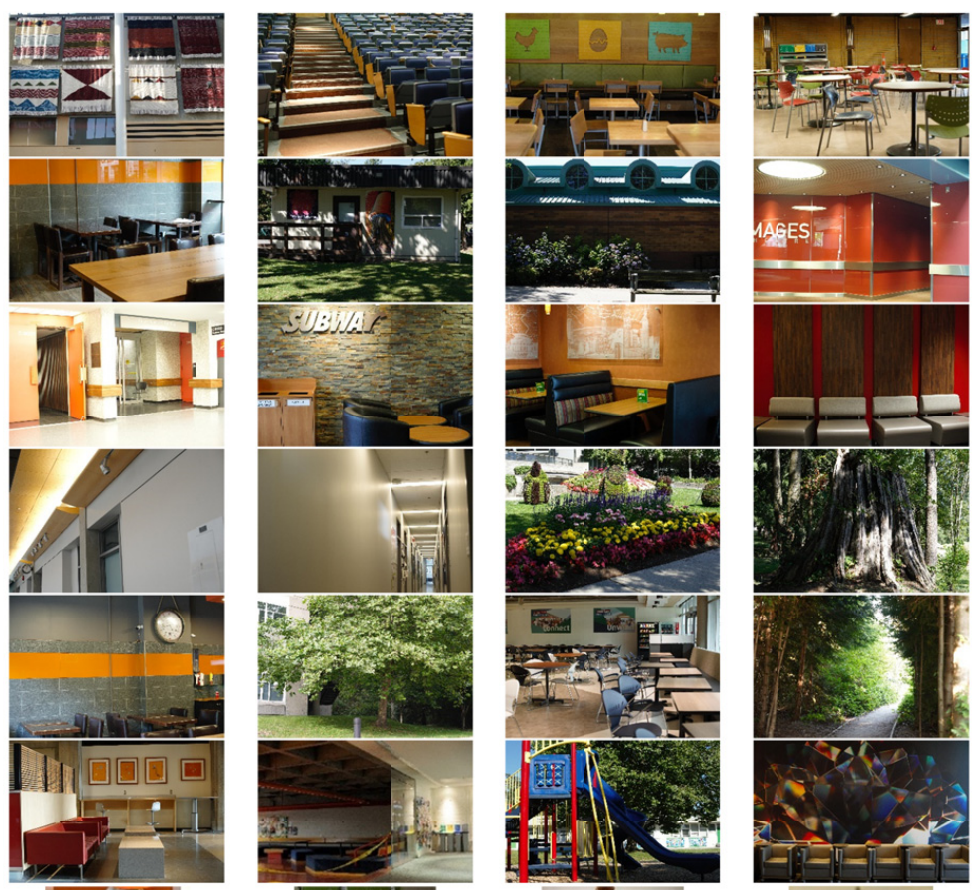
\includegraphics[width=0.4\textwidth]{img/sfu-dataset-sample.png}
        \caption{esempi di immagini del dataset SFU Gray Sphere.}
        \label{fig:sfu-dataset-sample}
      \end{figure}
    \end{frame}

    \begin{frame}
      \frametitle{sfu gray sphere drone}
      \begin{figure}[h]
        \centering
        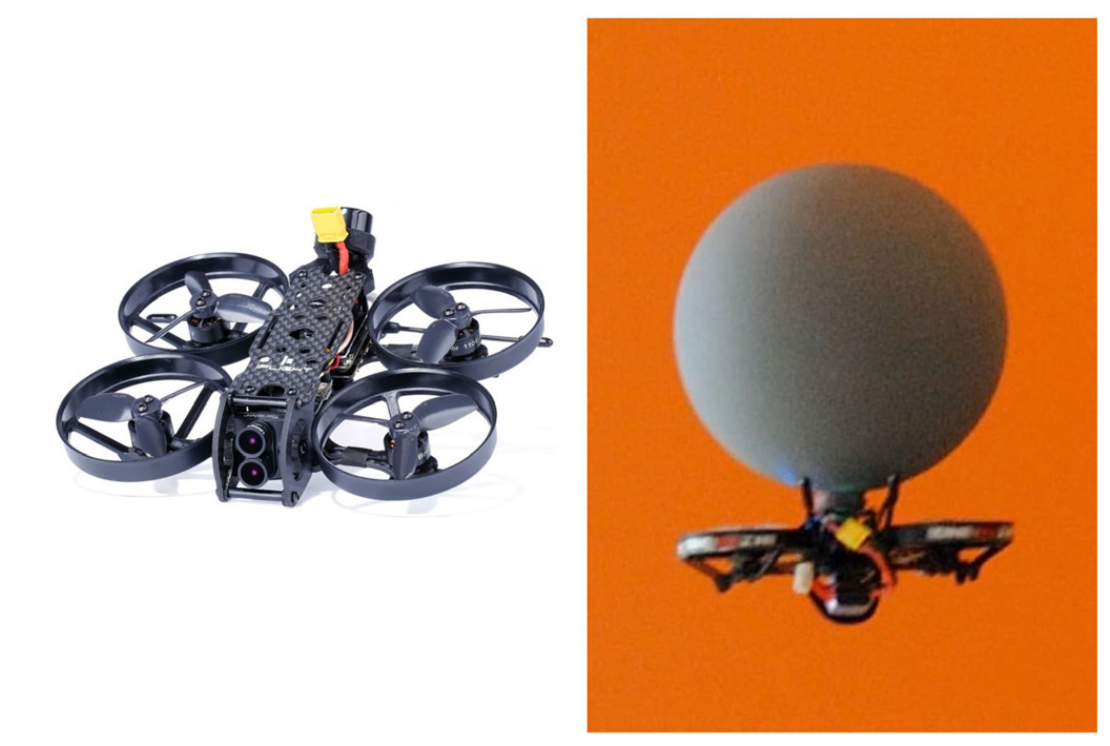
\includegraphics[width=0.6\textwidth]{img/sfu-drone.png}
        \caption{drone utilizzato per acquisire le immagini del dataset SFU Gray Sphere.}
        \label{fig:sfu-drone}
      \end{figure}
    \end{frame}

    \begin{frame}
      \frametitle{LSMI}

      \begin{figure}[h]
        \centering
        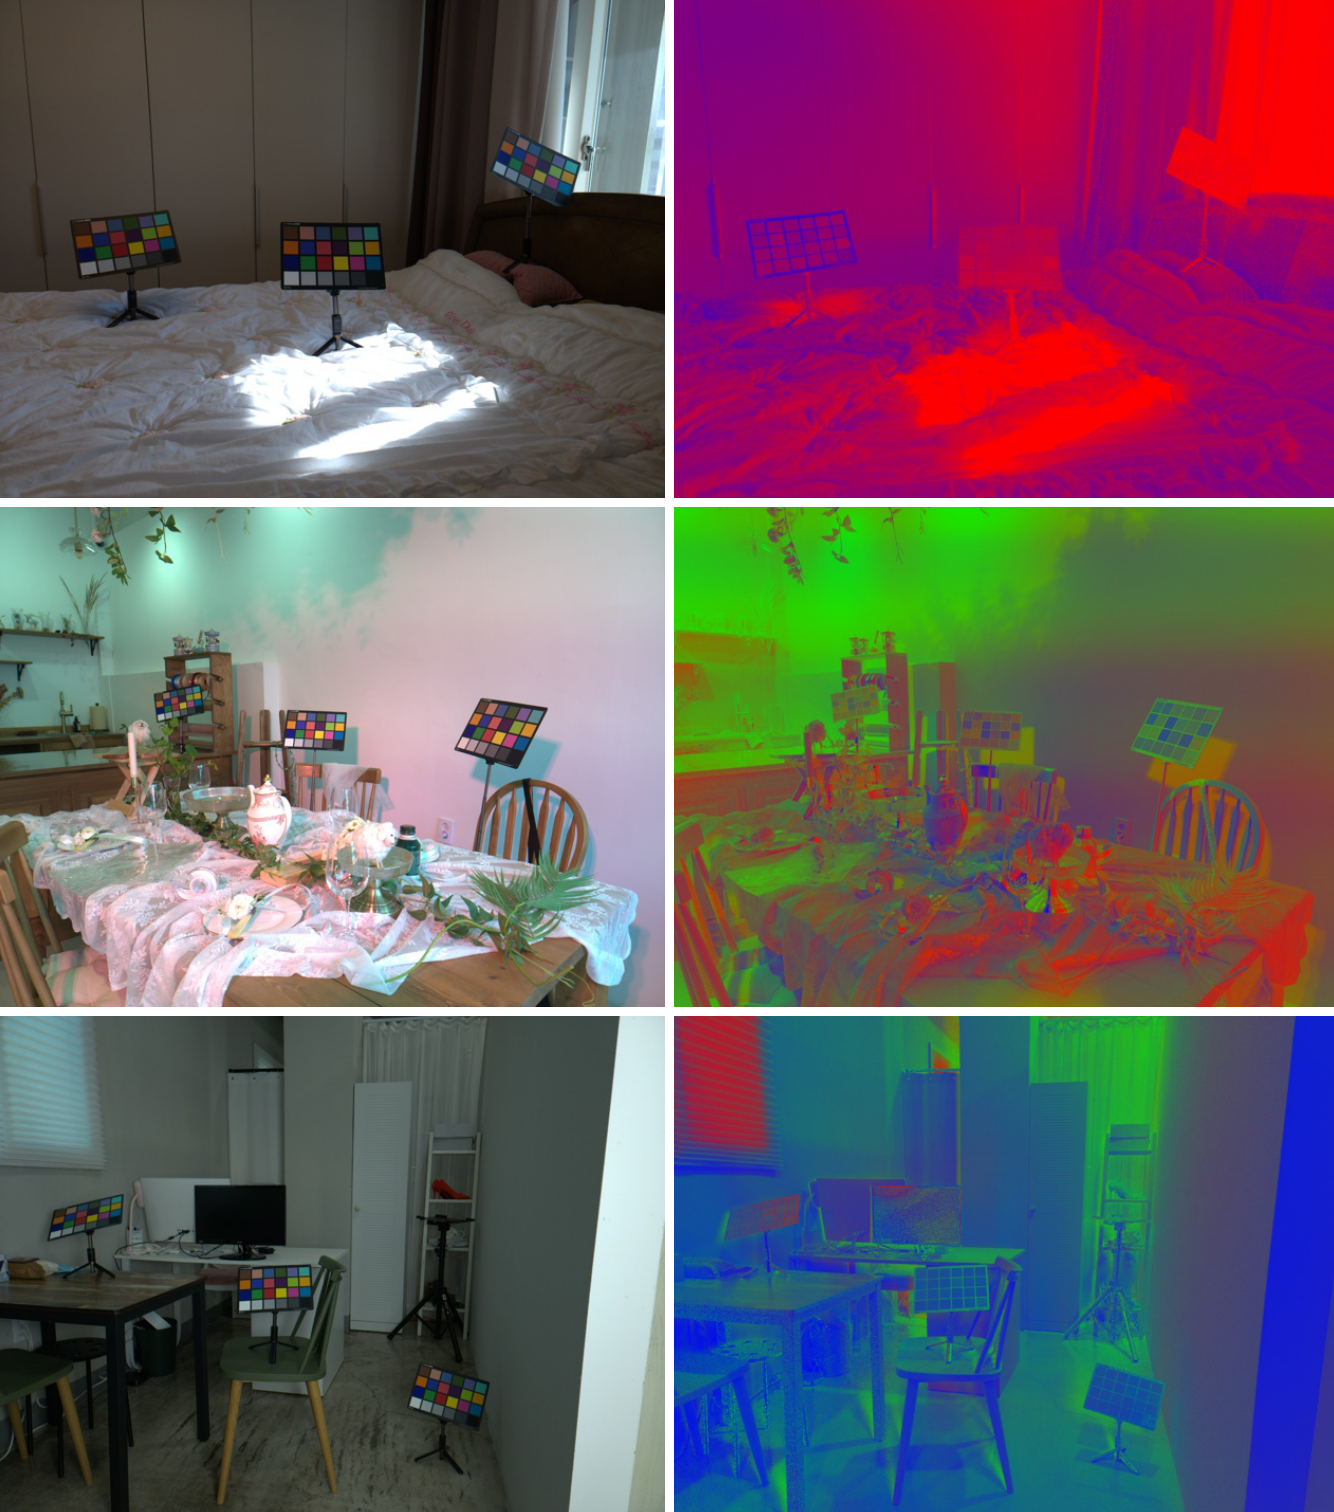
\includegraphics[width=0.3\textwidth]{img/lsmi-dataset-sample.png}
        \caption{esempi di immagini del dataset LSMI. Le immagini sono state acquisite con diversi dispositivi e mostrano scene con illuminazione variabile.}
        \label{fig:lsmi-dataset-sample}
      \end{figure}
    \end{frame}

     \begin{frame}
       \frametitle{Flying Gray Ball}

        \begin{figure}[h]
          \centering
          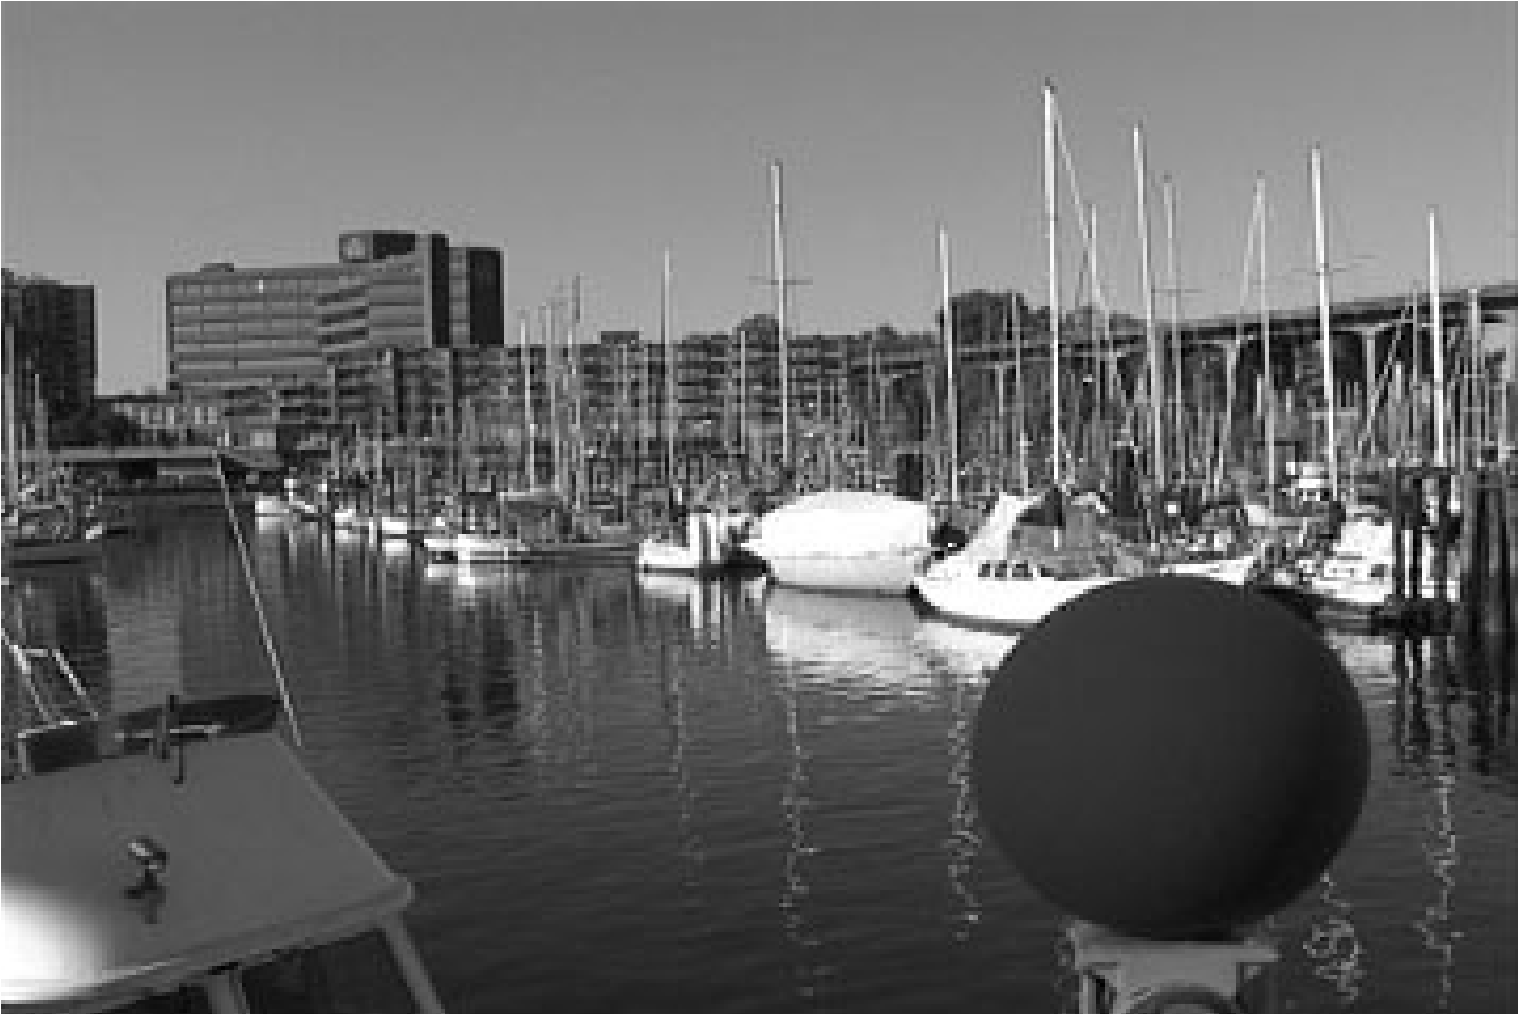
\includegraphics[width=0.6\textwidth]{img/flying-ball-dataset-sample.png}
          \caption{esempio di immagine del dataset Flying Gray Ball}
          \label{fig:flying-ball-dataset-sample}
        \end{figure}

    \end{frame}
    %
    % \begin{frame}
    %   \frametitle{colorchecker}
    %   \begin{itemize}
    %     \item<1-> scene sia in interno che in esterno
    %     \item<2-> un singolo illuminante globale
    %     \item<3-> ground truth: Macbeth ColorChecker + posizione gliglia grigia per ogni immagine
    %   \end{itemize}
    % \end{frame}
    %
    % \begin{frame}
    %   \frametitle{cube++}
    %   \begin{itemize}
    %     \item<1-> scene in esterno
    %     \item<2-> un singolo illuminante globale
    %     \item<3-> ground truth: Macbeth ColorChecker + bounding box della griglia
    %   \end{itemize}
    % \end{frame}
    %
  \section{References}
    \begin{frame}[allowframebreaks]
      \printbibliography
    \end{frame}
\end{document}
